%%%%%%%%%%%%%%%%%%%%%%%%%%%%%%%%%%%%%%%%%%%%%%%%%%%%%%%
% Please note that whilst this template provides a
% preview of the typeset manuscript for submission, it
% will not necessarily be the final publication layout.
%
% letterpaper/a4paper: US/UK paper size toggle
% num-refs/alpha-refs: numeric/author-year citation and bibliography toggle

%\documentclass[letterpaper]{oup-contemporary}
\documentclass[a4paper,num-refs]{oup-contemporary}

%%% Journal toggle; only specific options recognised.
%%% (Only "gigascience" and "general" are implemented now. Support for other journals is planned.)
\journal{gigascience}

\usepackage{graphicx}
\usepackage{siunitx}

%%% Flushend: You can add this package to automatically balance the final page, but if things go awry (e.g. section contents appearing out-of-order or entire blocks or paragraphs are coloured), remove it!
% \usepackage{flushend}

\title{Training Infrastructure as a Service}

%%% Use the \authfn to add symbols for additional footnotes, if any. 1 is reserved for correspondence emails; then continuing with 2 etc for contributions.
\author[1,\authfn{1},\authfn{2}]{Helena~Rasche}
\author[2,\authfn{2}]{Bj\"orn~Gr\"uning}

\affil[1]{Bioinformatics Group, Department of Computer Science, University of Freiburg, 79110 Freiburg im Breisgau, Germany}

%%% Author Notes
\authnote{\authfn{1}helena.rasche@gmail.com}
\authnote{\authfn{2}Contributed equally.}

%%% Paper category
\papercat{Technical Note}

%%% "Short" author for running page header
\runningauthor{Rasche and Gr\"uning}

%%% Should only be set by an editor
\jvolume{00}
\jnumber{0}
\jyear{2017}

\begin{document}

\begin{frontmatter}
\maketitle
\begin{abstract}
%The Abstract (250 words maximum) should be structured to include the following details: \textbf{Background}, the context and purpose of the study; \textbf{Results}, the main findings; \textbf{Conclusions}, brief summary and potential implications. Please minimize the use of abbreviations and do not cite references in the abstract.
\textbf{Background:} Hands-on training, whether it is in Bioinformatics or other scientific domains, requires significant resources and knowledge to setup and run.
Trainers must have access to infrastructure that can support the sudden spike in usage with classes of 30 students running sometimes resource intensive tools simultaneously.
The student jobs must run quickly and not wait in queues, lest they disrupt the timetable set out for the class. Often times this is achieved via running on a private server where there is no contention for the queue, but this requires the teacher to have the technical knowledge to manage this, in addition to their responsibilities teaching. This presents significant burdens to potential trainings, in terms of infrastructure cost, person-hours in preparation, technical knowledge, and available staff to manage such hands-on trainings.

\textbf{Findings:} Galaxy Europe has developed Training Infrastructure as a Service (TIaaS) which we provide to the scientific commnuity as a service built on top of the Galaxy Platform. Teachers request a training and UseGalaxy.eu administrators launch compute nodes in the cloud specifically for the training. Students are transparently placed in a private queue where their jobs run without delay. Teachers access the dashboard of the TIaaS Join Service and follow the progress of their students.

\textbf{Conclusions:} TIaaS provides reusable, free, and fast infrastructure for Galaxy training. The instructor dashboard provides visibility into class progress reducing the need for helpers who monitor students or self-reporting of progress. In the past 12 months, 55 trainings with over 1300 students have used this infrastructure for training across scientific domains, all enjoying the accessibility and reproducibility of Galaxy for training the next generation of bioinformaticians.
\end{abstract}

\begin{keywords}
Galaxy; Training; Teaching; Bioinformatics
\end{keywords}
\end{frontmatter}

\section{Findings}
\subsection{Background}

% The background section should be written in a way that is accessible to researchers without specialist knowledge in that area and must clearly state---and, if helpful, illustrate---the background to the research and its aims. The section should end with a brief statement of what is being reported in the article.

% todo: sentence about how importnt hands-on training is?
With the volume of bioinformatics data becoming available, the availability of training for bioinformaticians is not keeping up (\cite{Attwood2017}).
The Galaxy platform \cite{afgan2018galaxy} provides one such infrastructure on which to conduct trainings, it provides a user-friendly web-based interface to command line tools. With a wide range of tools across bioinformatics domains and beyond, and pre-existing popularity within the life sciences community (7000+ citations, 7200+ tools \cite{galaxycitations,galaxytoolshed}) it is an ideal platform for training students (\cite{gtn}).

The Galaxy community has developed a wide array of hands-on training materials covering the bioinformatics domains and beyond (\cite{training-site}) in an attempt to combat this issue, but in order to run these tutorials at scale, one occasionally needs access to significant resources. The quite popular ``Reference-based RNA-Seq data analysis'' tutorial uses the STAR aligner (\cite{Dobin2012}), and while an ultra-fast aligner is ideal during training, it also consumes 32-64 GB of RAM at minimum. Running a single copy of STAR might be fine, but having 30 students running it simultaneously can present unexpected delays.

Many tools across Galaxy have similar requirements, often based on input dataset sizes. If teachers choose to manage their own infrastructure they need to obtain this knowledge via testing the tutorial with multiple people simultaneously, and then configure their infrastructure to support the minimum memory and CPU requirements. If the instructor is also responsible for the compute infrastructure, any bugs which affect the training can become incredibly stressful events. Alternatively if the instructor chooses to use one of the many public Galaxy servers, they have someone else to blame if the server goes down, but their students' jobs could unexpectedly sit in shared queues for long periods of time. These can be significant barriers to would-be trainers who want to give a Galaxy or bioinformatics training course.

We developed Training Infrastructure as a Service (TIaaS) initially to make our own courses run more smoothly due to previous experiences with all of the aforementioned problems. TIaaS simply removes the main bottlenecks of training: setting up the training infrastructure is nearly completely automated, jobs are guaranteed to have private resources available so they can always run without delay, and it ensures separation of responsibilities between teachers who are teaching and the server administrators responsible for Galaxy Europe.

\subsection{Results}
\begin{figure}[bt!]
\centering
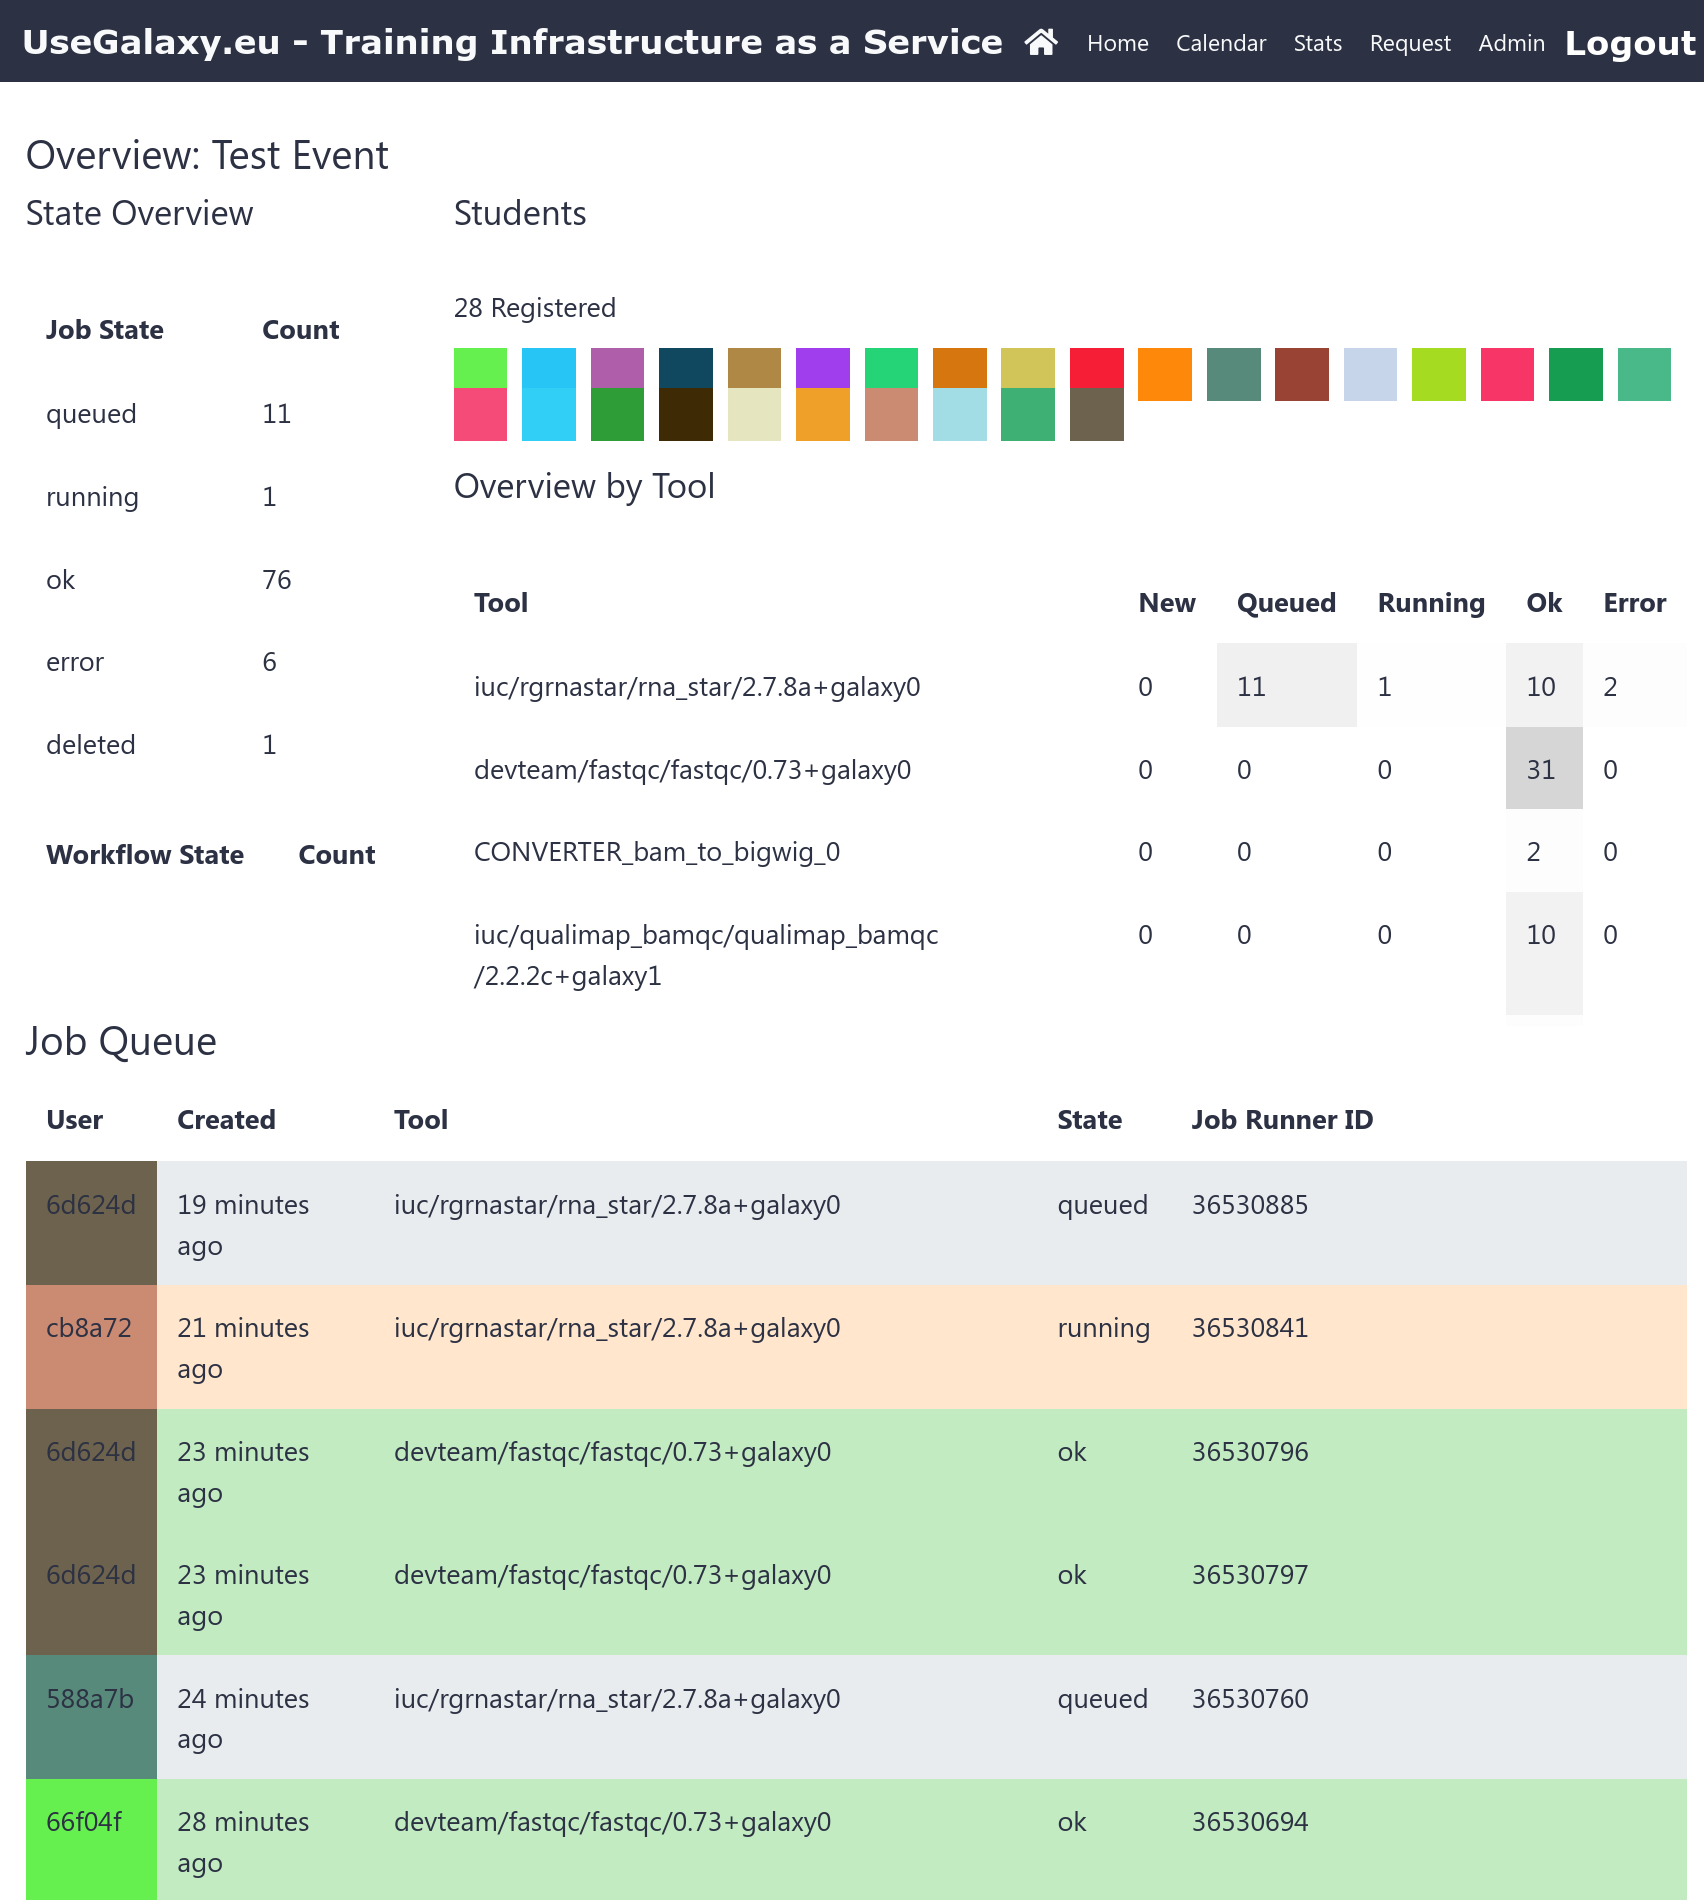
\includegraphics[width=\linewidth]{images/dashboard.png}
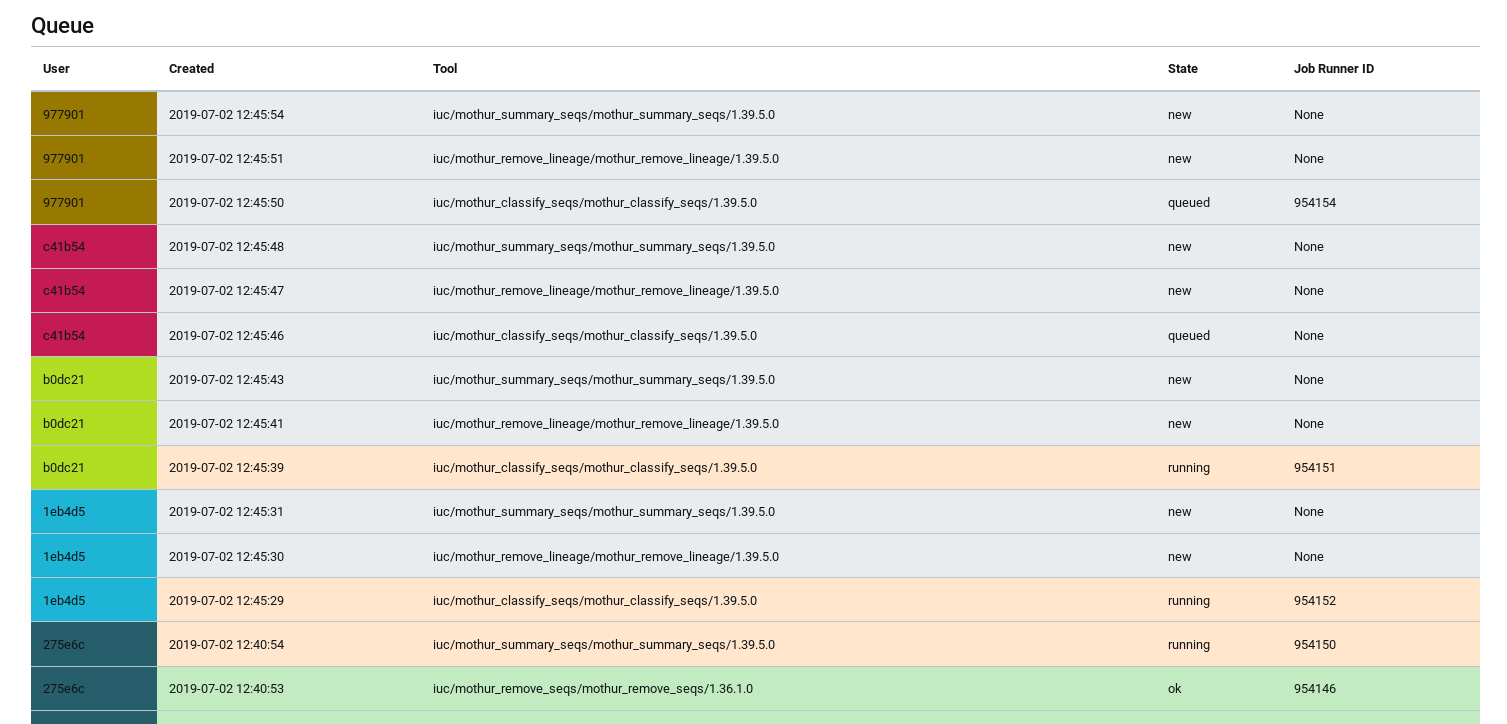
\includegraphics[width=\linewidth]{images/queue.png}
\caption{The top of the training dashboard page shows the status of the jobs in the past hours. A heatmap of the tools which were run indiciates if everything is running smoothly or if there is anything the teacher should look into. As students follow along and run different tools these show up, and complete, with approximately identical numbers of executions as students follow instructions. The bottom image shows the rest of the training dashboard, which lists jobs that were run chronologically, colour coded first by student, and second for the job status. Pseudorandom identifiers were originally used to protect user privacy as the dashboards were public, but even given the option to show more recognisable user identifiers was deemed to be distracting from the main purpose of a quick overview for teachers.}\label{figure:dashboard}
\end{figure}

We implemented a web service and some job scheduling rules which functions together to present a private queue for users in specific groups. Trainers register their course and teaching materials with a Google Form. Galaxy administrators review requests, and upon approval run a bash script which schedule compute node VMs to be launched in the cloud, registers the training with the Group Joining Service (GJS), and registers the training with job scheduler. Administrators receive a URL such as \url{https://usegalaxy.eu/join-training/test}, which they share with the trainer, and the trainer can then in turn provide to their students. The scheduler, now aware of the training group, will grant any job run by someone in that group the ability to run on the private training nodes (Figure \ref{figure:queue}).

\begin{figure}[bt!]
\centering
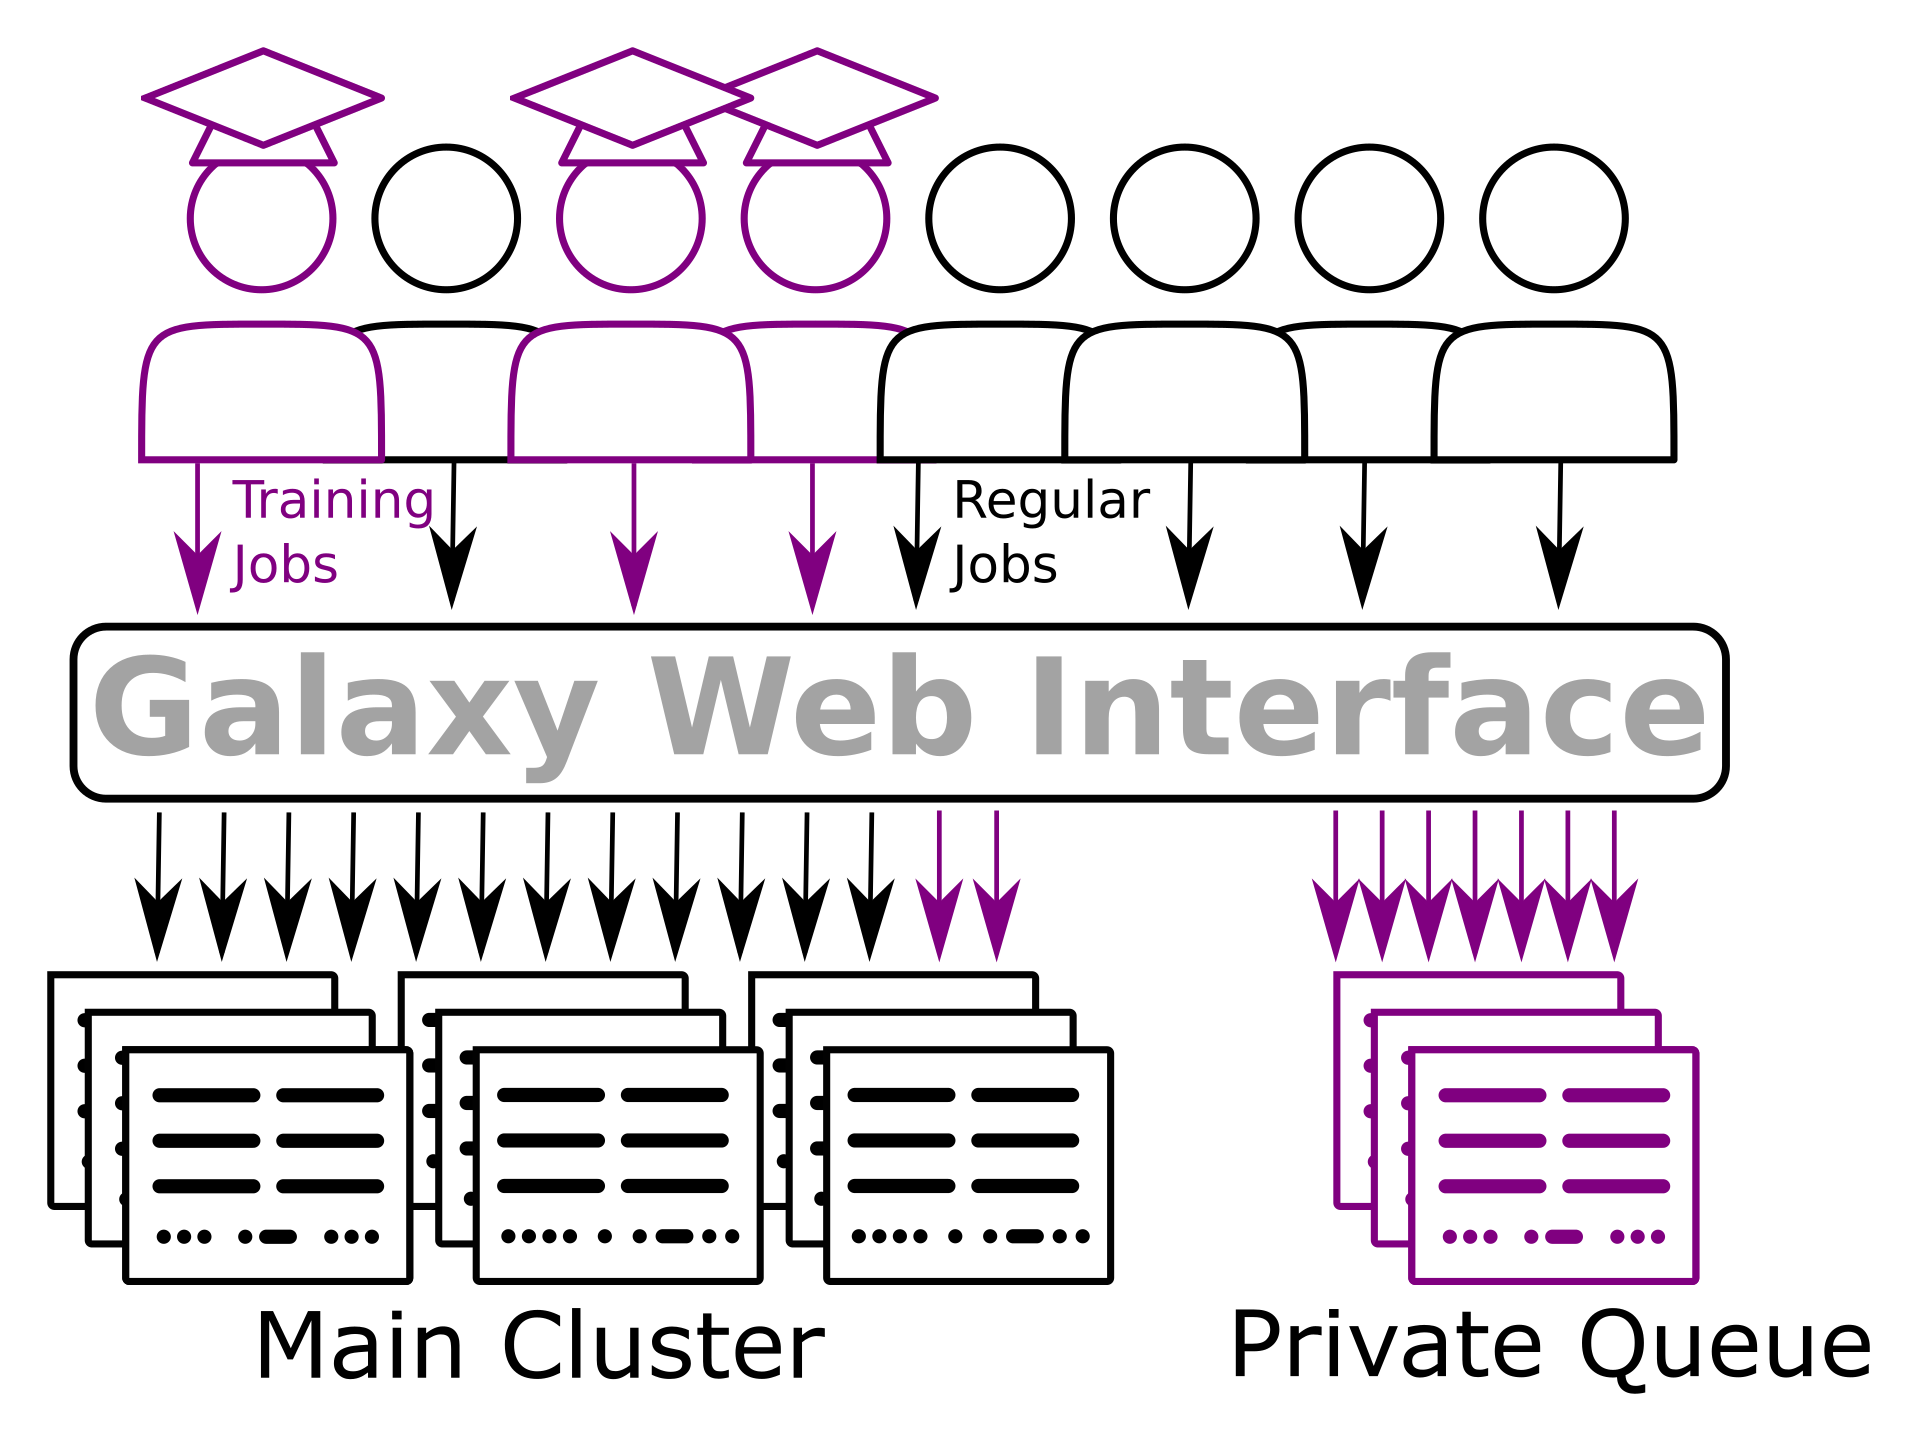
\includegraphics[width=\linewidth]{images/rules.png}
\caption{All jobs are processed by the same Galaxy server, but jobs from users in the training groups receive special handling. These jobs are allowed to run on the protected training resources (purple). If the training resource is full, these jobs can spill over to the main queue if necessary.}\label{figure:queue}
\end{figure}

The course dashboard, visualising the progress of students (Figure \ref{figure:dashboard}), has significantly eased the lives trainers. Previously Galaxy administrators received numerous messages during trainings, asking about student progress and if their jobs are running ok. The dashboard has nearly eliminated these by providing instantaneous feedback for the teachers into how their students are progressing. It has also enabled hybrid trainings to take place, where trainers present a topic via video and it is broadcast to numerous sites. Requiring multiple sites to give constant feedback on how students progress is not efficient or scalable, with the training dashboard this is unnecessary as trainers, helpers, and even students can see how everyone is progressing.

\subsubsection{Usage}
Since the introduction of TIaaS in July 2018, it has seen nearly constant use with more than 55 trainings occuring on the platform, all across the world (Figure \ref{figure:map}). Everything from one day workshops for bioinformaticians to multi-month courses for highschool students have been hosted by TIaaS and UseGalaxy.eu, covering topics such as HTS, RNA-Seq, ChIP-Seq, Imaging Analysis, Proteomics, and Machine Learning.

\begin{figure}[bt!]
\centering
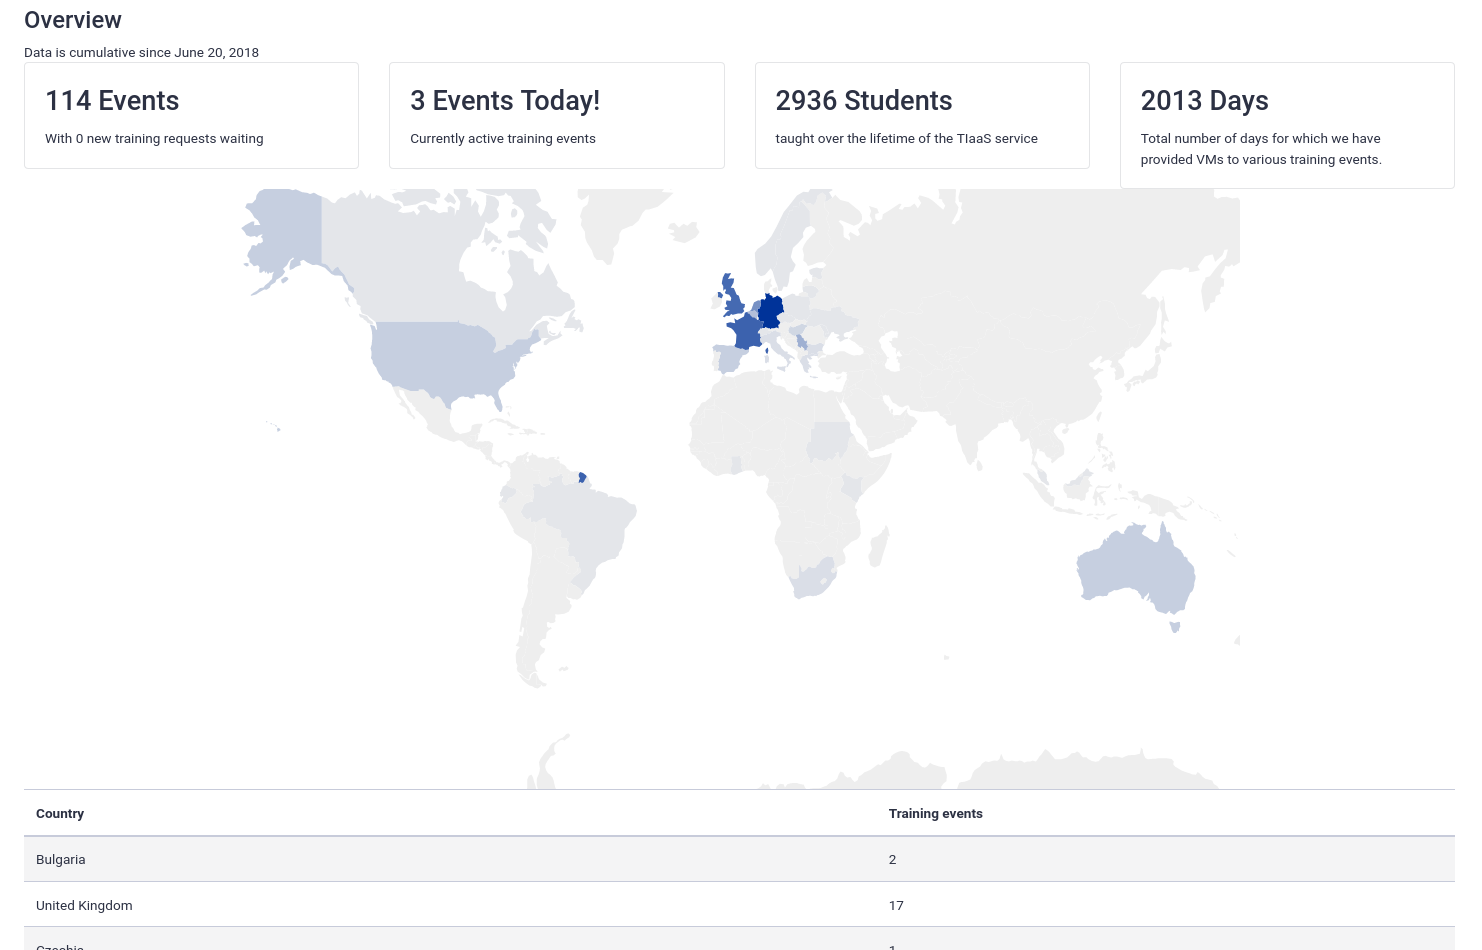
\includegraphics[width=\linewidth]{images/map.png}
	\caption{Since its introduction, TIaaS has seen worldwide usage despite--or perhaps in some cases due to--the server being hosted in Germany.}\label{figure:map}
\end{figure}

Class sizes have ranged considerably, from the median of 15 students to a maximum of 80 at a Transcriptomics workshop. Most course were quite short training events with a median of two days, however some ran for multiple months like a highschool course that used the service for three months, over the course of a semester, teaching Metagenomics.

\section{Methods}

\subsection{Implementation}
The Group Joining Service (GJS) was written in python using the Flask framework. It is a relatively small service, simply talking to the Galaxy DB first for user authentication and second to add incoming users to their training group when they visit their event-specific URL. When students visit the dashboard (e.g. joining a training named ``test'' with path \texttt{/join-training/test}), their Galaxy session cookie is decoded into their user ID, and then they are added to the group \texttt{training-test} within Galaxy. This group is automatically created on demand.

The student progress dashboard is part of the same service, accessed at a url like \url{https://usegalaxy.eu/join-training/test/status}, where \texttt{test} is the ``training identifier''. This view queries the Galaxy database for the users in the gr roup (e.g. \texttt{test}), and then fetches all jobs created by those users in the past N hours, before displaying these as a list and several summary tables to the viewer. The viewer can change the time range to view, or have the page auto-refresh if they want a more dynamic view into their class.

When a job is submitted by a user in a training group, UseGalaxy.eu's \href{Sorting Hat}{https://github.com/usegalaxy-eu/sorting-hat} system reads the user's groups and roles, and if any of these include something prefixed with \texttt{training-}, then this is converted to an HTCondor requirement string such as \texttt{GalaxyGroup == "training-test"} indicating to condor that it can run on any nodes which have a matching label.

\subsection{Reusability}
An Ansible role was produced for deploying the GJS, in order to simplify deployment at other sites. The routing rules unfortunately cannot easily be integrated into Galaxy itself, and must be re-implemented at other sites which wish to produce a similar setup. Galaxy provides the ability to talk to multiple cluster systems but unfortunately there is currently no generic abstraction for labelled nodes our the routing logic of HTCondor which we leverage for this private queueing.

\section{Availability of source code and requirements}

\begin{itemize}
\item Project name: ~Training Infrastructure as a Service
\item Github repository:~\url{https://github.com/usegalaxy-eu/tiaas-group-join/}
\item Training Manual: ~\url{https://training.galaxyproject.org/training-material/topics/instructors/tutorials/setup-tiaas-for-training/tutorial.html}
\item Operating system(s): ~Unix
\item Other requirements: ~Galaxy version 18.01 or higher
\item License: ~GNU AGPL-3.0
\end{itemize}

\section{Availability of supporting data and materials}
All code is open source and available on GitHub.

\section{Declarations}

\subsection{List of abbreviations}
%if abbreviations are used in the text they should be defined in the text at first use, and a list of abbreviations should be provided in alphabetical order.

\begin{itemize}
\item GJS: TIaaS Group Join Service
\item TIaaS: Training Infrastructure as a Service
\end{itemize}


\subsection{Competing Interests}
The authors declare that they have no competing interests.


\subsection{Funding}
This project was made possible with the support of the Albert Ludwig University of Freiburg
% TODO, deNBI elixir blah

\subsection{Author's Contributions}
HR and BG contributed to the tool development and writing of the manuscript.

\section{Acknowledgements}
The authors would like to thank the Galaxy community for their enthusiasm for this project, and their feedback on each iteration.

%% Specify your .bib file name here, without the extension
\bibliography{paper-refs}

\end{document}
